\subsection{Hough Transform} \label{add:hough_transform}

    \begin{wrapfigure}{r}{0.45\textwidth}
        \centering
        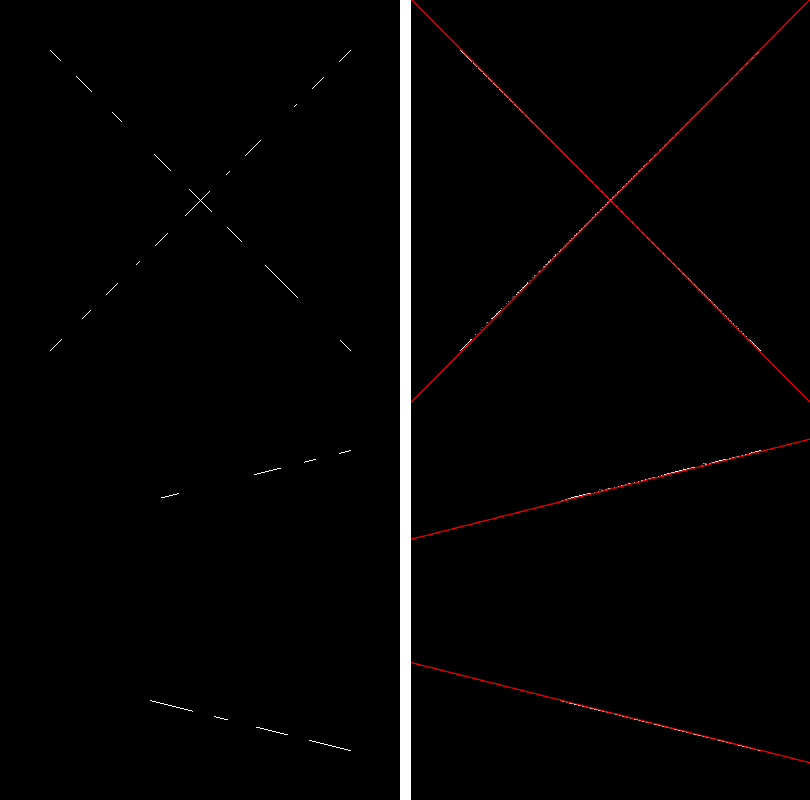
\includegraphics[width=1\textwidth]{hough_transform}
        \caption{\label{fig:hough_transform} Hough transform example. The red lines on the right image denote the lines found by the method.}
    \end{wrapfigure}

The Hough Transform is a method usually utilized to extract features in image analysis, originally proposed by Paul Hough~\cite{hough1962method}.
The method is used to detect simple shapes such as straight lines or circles in any set of points with given coordinates (usually from images) by finding groupings in these sets via a voting procedure over a set of parameterized properties.
An example of the detection of straight lines can be seen in Figure \ref{fig:hough_transform}.
In the left image the points are marked in white, while in the right image the lines found are marked in red.

For the case of detecting straight lines in two dimensions, the line is defined as $y = mx + b$ with its representation in its \textbf{Hessian normal form}~\cite{gellert2012vnr} is:
    \begin{equation*}
        r = x\cos{\theta} + y\sin{\theta}\,,
    \end{equation*}
where $r$ is the distance from the origin to the closest point in the line and $\theta$ is the angle between the $x$ axis and the line.
Given a point in the plane, the set of all lines going through that point corresponds to a sinusoidal curve in the $(r,\theta)$ plane.
A set of more than one point that form a straight line will produce multiple sinusoids crossing at the $(r,\theta)$ plane for that line, and thus, the original problem of detecting collinear points can be expressed as the problem of finding concurrent curves.